\\
دستگاه زیر را درنظر بگیرید:
\begin{center}
    \begin{cases}
      x_1 - x_3 = 0.2\\
      - 1/2x_1 + x_2 + 1/4x_3 = -1.425\\
      x_1 - 1/2x_2 + x_3 = 2
    \end{cases}
\end{center}

پاسخ این دستگاه به‌صورت
$(0.9, −0.8, 0.7)^t$
است.
\begin{enumerate}
\item
از تقریب اولیه‌ی $x^{(0)}$ و روش گاوس-سایدل استفاده کنید و پاسخ را با خطای
$10^{-2}$
و در حداکثر ۳۰۰ تکرار به‌دست آورید.
\item
در‌صورتی‌که دستگاه را به شکل زیر تغییر دهیم، پاسخ بخش الف چه خواهد شد؟
\begin{center}
$
	\begin{cases}
      	x_1 - 2x_3 = 0.2\\
      	- 1/2x_1 + x_2 - 1/4x_3 = -1.425\\
      	x_1 - 1/2x_2 + x_3 = 2
    	\end{cases}
    $
\end{center}
\end{enumerate}

\textcolor{blue}{
حل
\\
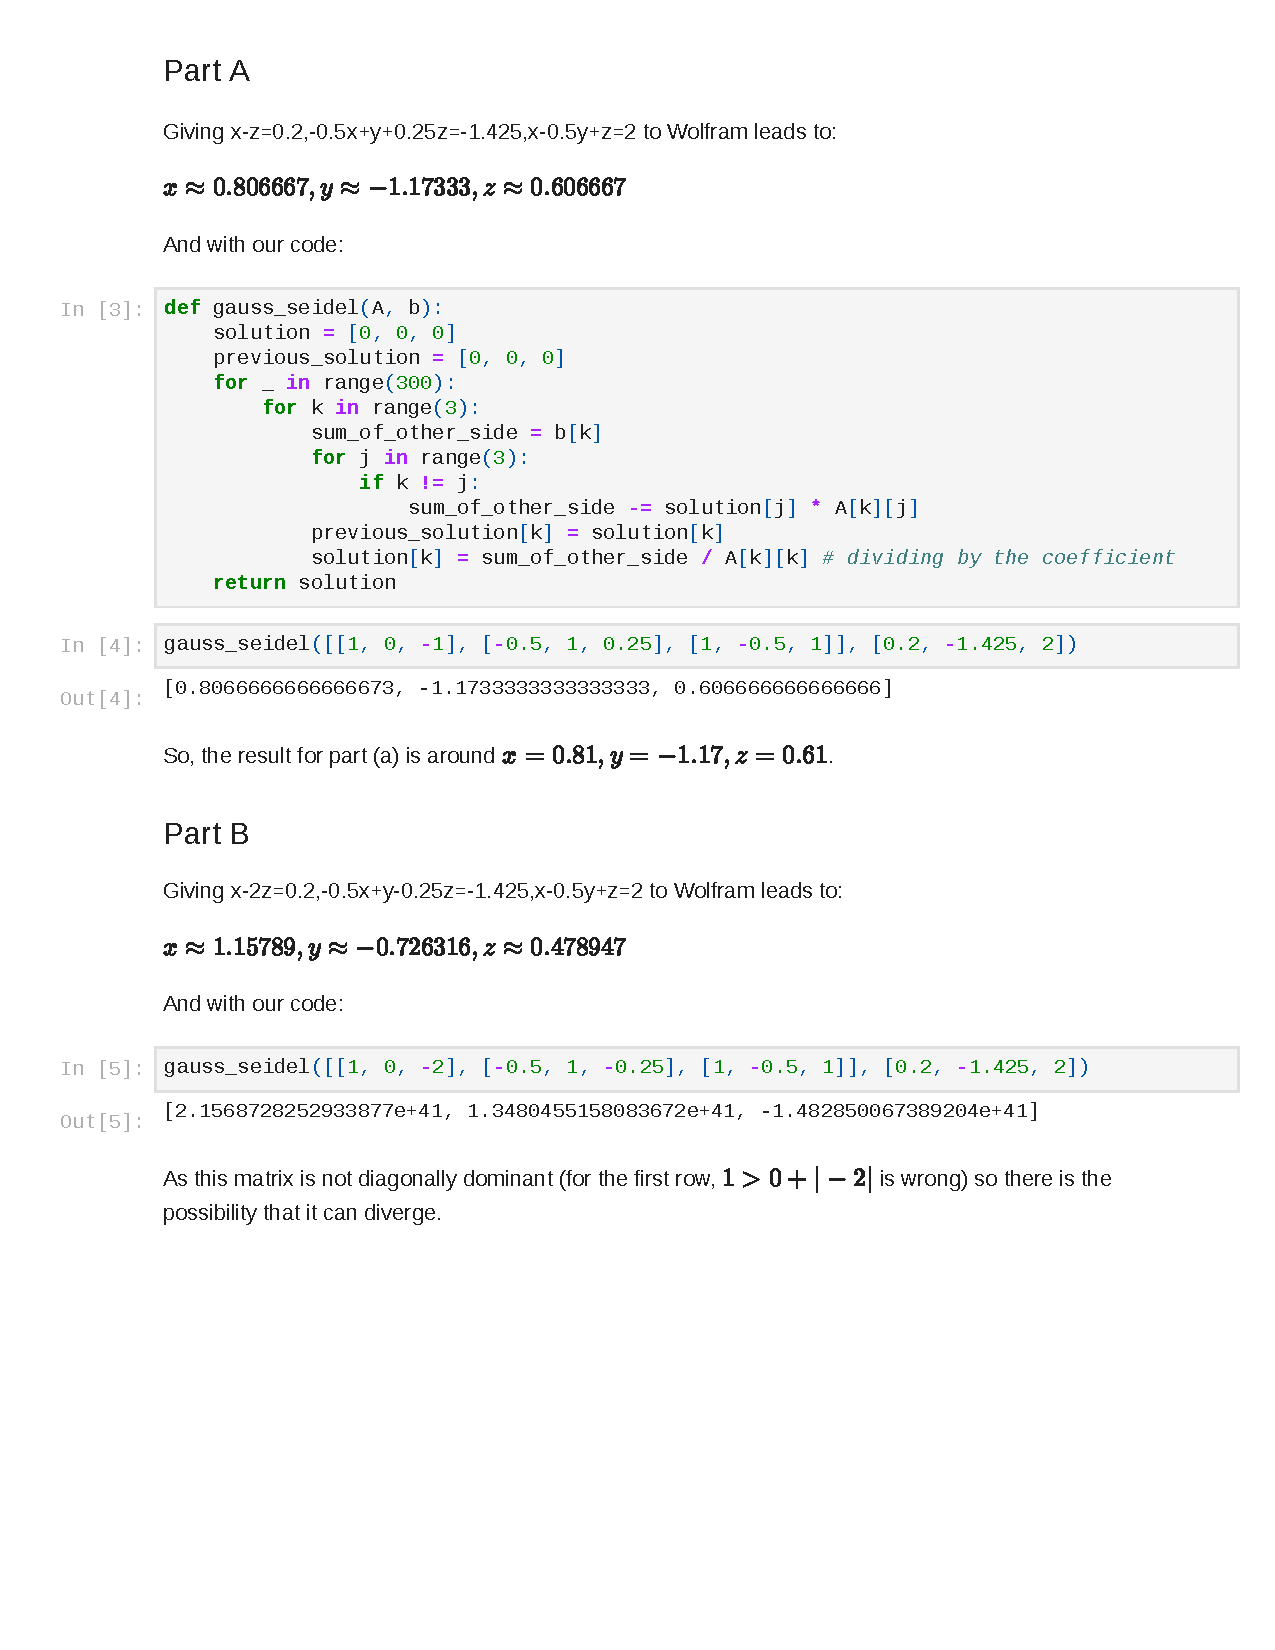
\includepdf[pages={1-},scale=1]{q4.pdf}
}